% +--------------------------------------------------------------------+
% | Sample Chapter 2
% +--------------------------------------------------------------------+

\cleardoublepage

% +--------------------------------------------------------------------+
% | Replace "This is Chapter 2" below with the title of your chapter.
% | LaTeX will automatically number the chapters.                      
% +--------------------------------------------------------------------+

\chapter{Background}
\label{makereference2}

Two pieces of apparatus were used to conduct the experiments in this thesis. This chapter will detail the purpose, design and recreation of the equipment. Section ~\ref{makereference2.1} will cover the new Motorlab, including the hardware implementation, design of components, and basic functionality. Section ~\ref{makereference2.1.1} will detail how a new type of position sensor works that is used for the position measurements of the Motorlab. Then, the older Motorlab will be discussed and compared to the new Motorlab in section ~\ref{makereference2.2}.

\section{New Motorlab}
\label{makereference2.1} 

The new Motorlab is a reimplementation of older laboratory hardware created by Dr. Schinstock and Dr. White for Control of Mechanical Systems I at Kansas State University. The Motorlab allows users to connect the theoretical ideas of control theory with those in practice. 


\subsection{Position Sensor}
\label{makereference2.1.1} 


The encoder that is being used on the Motorlab consists of 14-bit on-axis magnetic rotary position sensor chip, specifically the AS5047D by AMS. The position sensor chip provides high resolution absolute angle measurements (roughly 2000 steps per revolution) through a full 360 degree range. In addition to the fast absolute angle measurement system that the position sensor provides, it also has \ac{DAEC} that provides position control systems with near 0 latency \citep{1}.  

The AS5047D chip is a magnetic sensor that utilizes the Hall-effect. The chip works by taking the Hall sensors and converting the perpendicular magnetic field on the surface of the chip to a voltage. The voltage signals are filtered and amplified in order to calculate the angle of the magnetic vector. In order for position measurements to be taken, a small diametrically opposed magnet must be placed on the shaft of the equipment being measured. The magnet and AS5047D are contactless, meaning there is a small air gap between the chip and magnet. As the magnet rotates above the chip (Figure~\ref{magnet_rotation}), angle measurements are calculate and transmitted through the chip. The Motorlab uses the AS5047D chip primarily as a position and speed control system. 

\begin{figure}[htb]%t=top, b=bottom, h=here
\begin{center}
    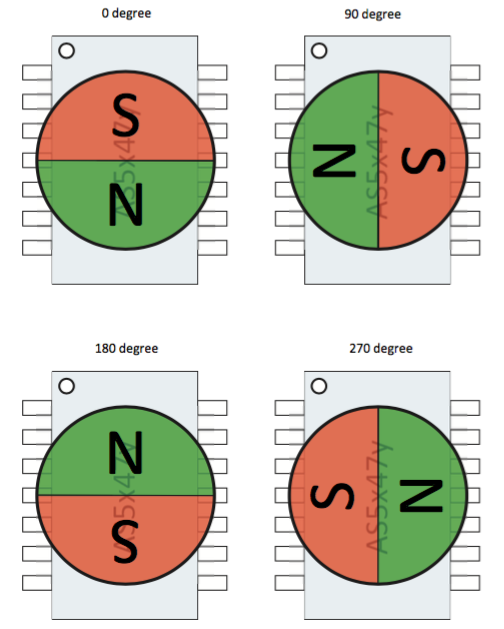
\includegraphics[height=4in]{figures/magnetic_field.png}

    \caption[Magnet and AS5047D]{Magnet and AS5047D}

    \label{magnet_rotation}
\end{center}
\end{figure}

\subsection{Motorlab Parts}
\label{makereference2.1.2} 

\begin{figure}[htb]%t=top, b=bottom, h=here

    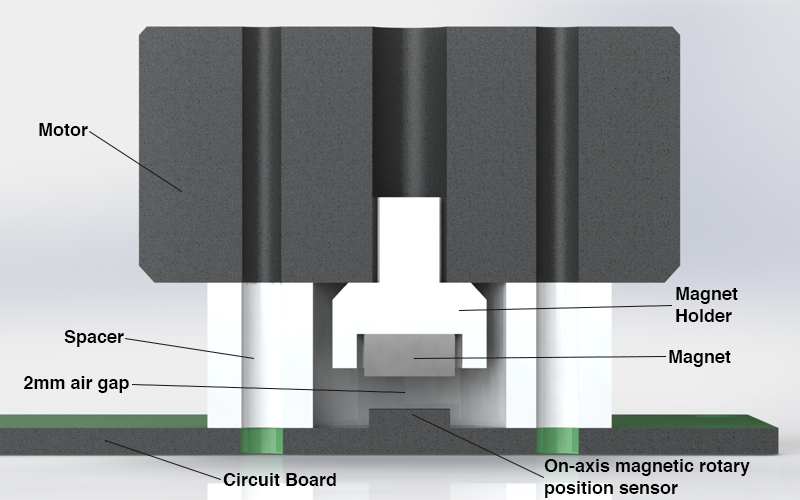
\includegraphics[height=4in]{figures/section_view_motorlab_assembly.png}

    \caption[Section View of Motorlab Assembly]{Section View of Motorlab Assembly}

    \label{section_view_motorlab}
\end{figure}


\section{Old Motorlab}
\label{makereference2.2} 

Need information here